\documentclass{article}
\usepackage[paperwidth=7.2in,paperheight=2.25in,margin=0.05in]{geometry}
\usepackage{tikz}
\usetikzlibrary{arrows.meta,positioning,fit}
\pagestyle{empty}
\begin{document}
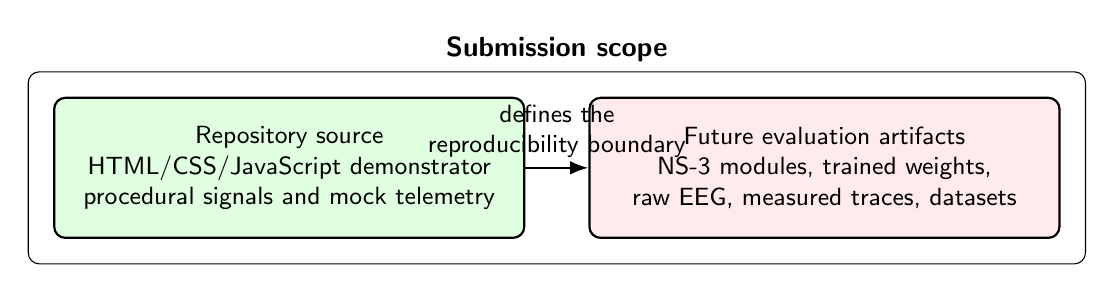
\begin{tikzpicture}[font=\sffamily\small, >=Latex, node distance=5mm and 8mm,
  avail/.style={draw, rounded corners, align=center, minimum width=2.35in, minimum height=0.7in, fill=green!12, thick},
  future/.style={draw, rounded corners, align=center, minimum width=2.35in, minimum height=0.7in, fill=red!8, thick},
  arrow/.style={->, thick}]
  \node[avail] (source) {Repository source\\HTML/CSS/JavaScript demonstrator\\procedural signals and mock telemetry};
  \node[future, right=of source] (evidence) {Future evaluation artifacts\\NS-3 modules, trained weights,\\raw EEG, measured traces, datasets};
  \draw[arrow] (source) -- node[above, align=center] {defines the\\reproducibility boundary} (evidence);
  \node[draw, rounded corners, fit=(source)(evidence), inner sep=9pt, label={[font=\bfseries\sffamily]above:Submission scope}] {};
\end{tikzpicture}
\end{document}
